\subsection{Resultados generales}
 En todas nuestras pruebas en valor de $MSS$ obtenido fue de $1452$ bytes, pero lo calculamos programáticamente antes de cada test para asegurarnos de usar el real en cada sistema utilizado.
 
 Establecimos como umbral del ZRTT el valor de $1$, ya que en el cálculo del mismo se efectúa una normalización a la distribución normal, y por definicion de esta un valor por fuera de este umbral comienza a ser estadísticamente relevante (solo un 15\% de los valores caen por encima del mismo).
 
\subsection{Estimación de RTT y análisis de parámetros}

A continuación presentamos los resultados de las pruebas de $\alpha$ y $n$ en función del RTT estimado para cada una de las universidades a las que realizamos un traceroute.

~

\begin{minipage}{0.48\textwidth}
    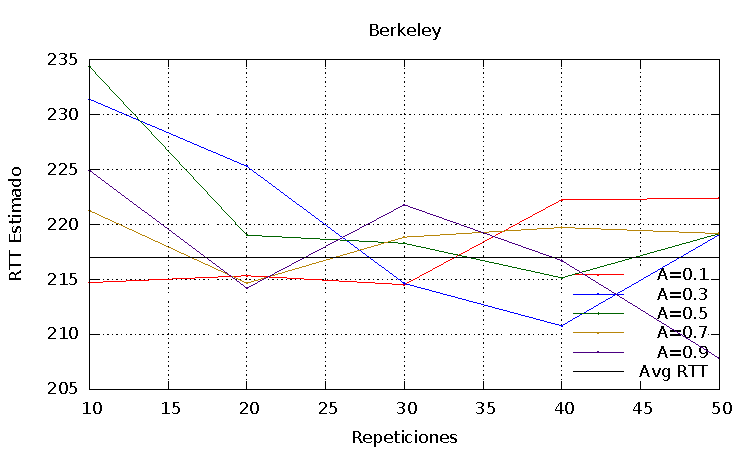
\includegraphics[scale=0.62]{imgs/thoughput/berkeley_rtt.pdf}
\end{minipage}
\begin{minipage}{0.48\textwidth}
    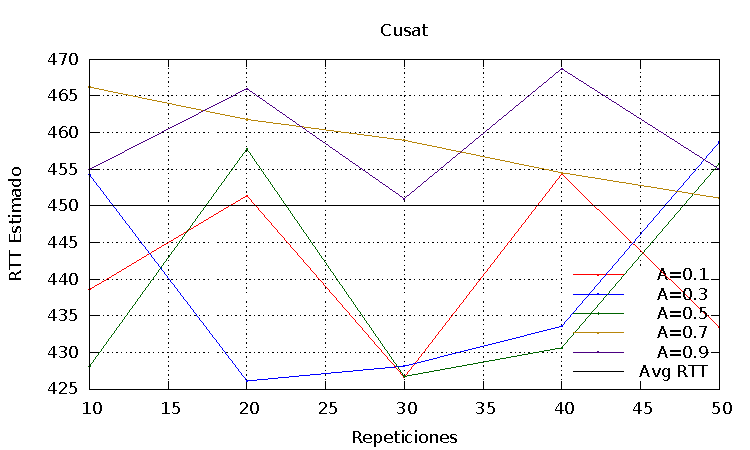
\includegraphics[scale=0.62]{imgs/thoughput/cusat_rtt.pdf}
\end{minipage}

\begin{minipage}{0.48\textwidth}
    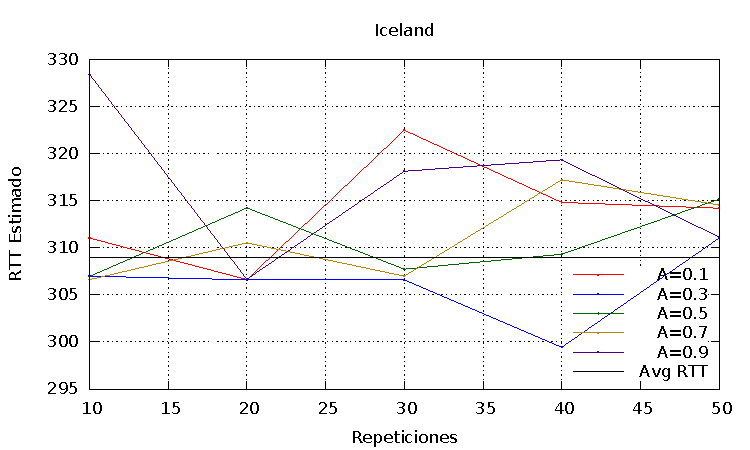
\includegraphics[scale=0.62]{imgs/thoughput/hi_rtt.pdf}
\end{minipage}
\begin{minipage}{0.48\textwidth}
    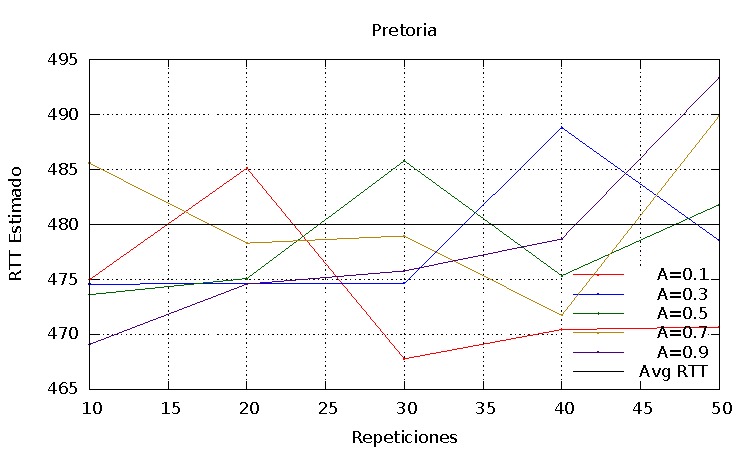
\includegraphics[scale=0.62]{imgs/thoughput/pretoria_rtt.pdf}
\end{minipage}

~

\begin{figure}[htp]
 \centering
 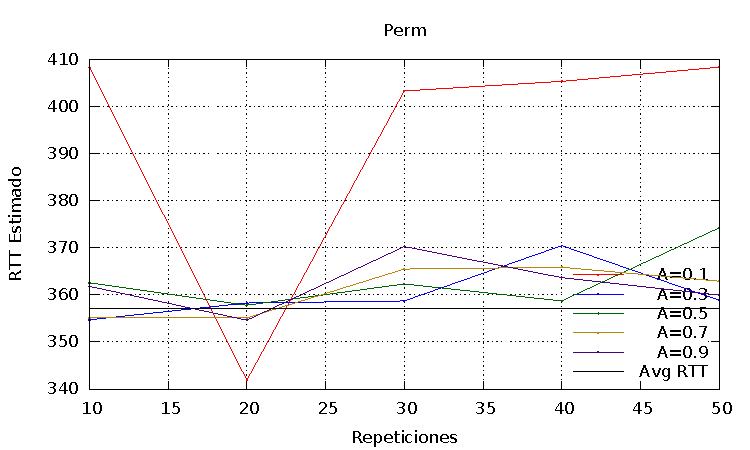
\includegraphics[scale=0.80]{imgs/thoughput/psu_rtt.pdf}
\end{figure}

%TODO: Laski - Completar aca con mas justificaciones sobre la eleccion de estos parametros. En los datos no veo que estos valores maximicen en throughput, por lo que no lo escribi como justificiacion.
Como se puede observar, en la mayoria de los casos $\alpha = 0.5$ y $n = 50$ estan cerca del promedio de RTT; lo que tiene sentido ya que con dichos valores las operaciones realizadas con los RTT se acercan bastante a el promedio. Por lo que, decidimos utilizar los mismos para la estimación de throughput.

\subsection{Berkeley, EEUU}

\begin{tabular}{|c@{\hspace{5ex}}c@{\hspace{5ex}}c@{\hspace{5ex}}c@{\hspace{5ex}}c|}
 \hline
 \rule{0pt}{1.2em}IP & ZRTT & AVG\_RTT & PAIS & CIUDAD\\[0.2em]
 \hline

\rule{0pt}{1.2em} 192.168.2.1  &  0.65 & 35.35 & (Private Address) & (Private Address) \\[0.2em]
\rule{0pt}{1.2em} 200.89.164.137  &  -0.11 & 46.40 & ARGENTINA & Buenos Aires \\[0.2em]
\rule{0pt}{1.2em} 200.89.165.130  &  -0.41 & 43.80 & ARGENTINA & Buenos Aires \\[0.2em]
\rule{0pt}{1.2em} 200.89.165.222  &  -0.27 & 47.29 & ARGENTINA & Buenos Aires \\[0.2em]
\rule{0pt}{1.2em} 208.178.195.205  &  -0.43 & 43.57 & ARGENTINA & Buenos Aires \\[0.2em]
\rule{0pt}{1.2em} 67.17.68.234  &  2.86 & 191.77 & UNITED STATES & Miami \\[0.2em]
\rule{0pt}{1.2em} 4.68.111.121  &  -1.44 & 141.79 & UNITED STATES & Miami \\[0.2em]
\rule{0pt}{1.2em} 4.35.156.66  &  1.07 & 207.65 & UNITED STATES & Los Angeles \\[0.2em]
\rule{0pt}{1.2em} 137.164.11.1  &  -0.2& 214.70 & UNITED STATES & Los Angeles \\[0.2em]
\rule{0pt}{1.2em} 137.164.46.144  &  -0.31 & 216.72 & UNITED STATES & Los Angeles \\[0.2em]
\rule{0pt}{1.2em} 137.164.50.31  &  -0.34 & 217.22 & UNITED STATES & Los Angeles \\[0.2em]
\rule{0pt}{1.2em} 128.32.0.37  &  -0.28 & 220.53 & UNITED STATES & Berkeley, CA \\[0.2em]
\rule{0pt}{1.2em} 128.32.0.101  &  -0.46 & 215.66 & UNITED STATES & Berkeley, CA \\[0.2em]
\rule{0pt}{1.2em} 169.229.216.200  &  -0.31 & 217.43 & UNITED STATES & Berkeley, CA \\[0.2em]
\hline
 \end{tabular}

\vspace{20pt}

Podemos observar el fenómeno ya mencionado sobre RTTs menores en saltos posteriores. En el gráfico de barras se puede observar que por encima del umbral quedan registrados dos saltos que corresponden a las distancias mas grandes segun la geolocalización. Sin embargo, el salto correspondiente al cable trasatlántico entre Buenos Aires y Miami (lugar del llamado NOC de las Américas) queda muy por encima del resto, evidenciando su utilización.

~

El valor del throughput estimado para esta ruta fue de $6.6$ kBps, el mayor de todas las rutas. Creemos que como el throughput esta relacionado intimamente con los valores de RTT, el valor alto de throughput es una consecuencia de la cercania del objetivo. El valor fue calculado utilizando $\alpha = 0.5$, $n = 50$ y un valor de EPLP de 1, que obtuvimos realizando 100 echo requests.

\begin{verbatim}
 --- berkeley.edu ping statistics ---
100 packets transmitted, 100 received, 0% packet loss, time 99134ms
rtt min/avg/max/mdev = 188.277/190.789/213.277/3.612 ms
\end{verbatim}

\begin{figure}[htp]
 \centering
 \includegraphics[scale=0.50]{imgs/berkeley.png}
\end{figure}


\begin{figure}[htp]
 \centering
  \includegraphics[width=5in]{imgs/maps/berkeley.png}
\end{figure}

\FloatBarrier
\subsection{Cochin, India}

\begin{tabular}{|c@{\hspace{5ex}}c@{\hspace{5ex}}c@{\hspace{5ex}}c@{\hspace{5ex}}c|}
 \hline
 \rule{0pt}{1.2em}IP & ZRTT & AVG\_RTT & PAIS & CIUDAD\\[0.2em]
 \hline

\rule{0pt}{1.2em} 192.168.2.1  &  -0.01 & 35.71 & (Private Address) & (Private Address) \\[0.2em]
\rule{0pt}{1.2em} 200.89.164.181  &  -0.33 & 45.44 & ARGENTINA & Buenos Aires \\[0.2em]
\rule{0pt}{1.2em} 200.89.165.150  &  -0.43 & 43.95 & ARGENTINA & Buenos Aires \\[0.2em]
\rule{0pt}{1.2em} 195.22.220.152  &  -0.42 & 44.05 & ARGENTINA & Buenos Aires \\[0.2em]
\rule{0pt}{1.2em} 195.22.216.142  &  1.12 & 213.52 & UNITED STATES & New Orleans \\[0.2em]
\rule{0pt}{1.2em} 195.22.216.142  &  -0.43 & 212.45 & UNITED STATES & New Orleans \\[0.2em]
\rule{0pt}{1.2em} 195.22.195.102  &  1.59 & 434.06 & ITALY & Milano \\[0.2em]
\rule{0pt}{1.2em} 218.248.235.161  &  -1.76 & 286.69 & INDIA & Bangalore \\[0.2em]
\rule{0pt}{1.2em} 210.212.233.50  &  1.10 & 454.65 & INDIA & Cochin \\[0.2em]
\rule{0pt}{1.2em} 210.212.233.50  &  -0.41 & 455.32 & INDIA & Cochin \\[0.2em]
\hline
 \end{tabular}

\vspace{20pt}

En una primera instancia, notamos que el IP \verb|195.22.220.152| fue marcado como Italiano pero su RTT era demasiado bajo. Verificando contra otras bases de localizacion de IP, comprobamos que efectivamente el nodo se encuentra en Argentina, si bien su rango pertenece a Italia, ya que el ISP dueño es una corporacion Italiana.

~

Nuevamente vemos una correspondencia entre el salto más largo, trasatlántico esta vez, y la diferencia entre RTTs, reflejada a su vez por el valor de ZRTT. Sin embargo también vemos una diferencia similar entre dos puntos supuestamente cercanos, y una diferencia negativa entre dos puntos supuestamente alejados. Sospechamos que esto último puede ser algún defecto en las bases de datos de geolocalización.

~

En este caso hay 3 saltos que quedan por encima del umbral, como se puede observar en el gráfico de barras. El primero de ellos corresponde al salto entre Buenos Aires y New Orleans, el segundo al salto entre New Orleans e Italia y el tercero corresponde al salto entre Italia e India. Los primeros dos seguramente involucren el uso de un cable trasatlántico.

~

% TODO: Revisar que la unidad del throughput este bien.
El valor del throughput estimado para esta ruta fue de $3.2$ kBps. Comparándolo con el anterior, podemos ver que el valor absoluto de RTT de la ruta sea mucho mayor afecta directamente al throughput obtenido, ya que los valores de $EPLP$ y $MSS$ se mantienen iguales. El valor fue calculado utilizando $\alpha = 0.5$, $n = 50$ y un valor de EPLP de 1, que obtuvimos realizando 100 echo requests.

\begin{verbatim}
--- cusat.ac.in ping statistics ---
100 packets transmitted, 100 received, 0% packet loss, time 99110ms
rtt min/avg/max/mdev = 420.858/422.976/433.482/1.565 ms
\end{verbatim}

\begin{figure}[htp]
 \centering
 \includegraphics[scale=0.5]{imgs/cusat.png}
\end{figure}

\begin{figure}[htp]
 \centering
  \includegraphics[width=5in]{imgs/maps/cusat.png}
\end{figure}

\FloatBarrier
\subsection{Reykjavik, Iceland}

\begin{tabular}{|c@{\hspace{5ex}}c@{\hspace{5ex}}c@{\hspace{5ex}}c@{\hspace{5ex}}c|}
\hline
\rule{0pt}{1.2em}IP & ZRTT & AVG\_RTT & PAIS & CIUDAD\\[0.2em]
\hline

\rule{0pt}{1.2em} 192.168.2.1  &  0.53 & 37.3 & (Private Address) & (Private Address) \\[0.2em]
\rule{0pt}{1.2em} 200.89.164.153  &  -0.24 & 45.36 & ARGENTINA & Buenos Aires \\[0.2em]
\rule{0pt}{1.2em} 200.89.165.130  &  -0.42 & 44.90 & ARGENTINA & Buenos Aires \\[0.2em]
\rule{0pt}{1.2em} 200.89.165.222  &  -0.36 & 47.18 & ARGENTINA & Buenos Aires \\[0.2em]
\rule{0pt}{1.2em} 208.178.195.205  &  -0.48 & 43.77 & ARGENTINA & Buenos Aires \\[0.2em]
\rule{0pt}{1.2em} 67.16.139.18  &  3.11 & 211.71 & UNITED STATES & Miami \\[0.2em]
\rule{0pt}{1.2em} 213.248.76.189  &  -1.33 & 168.31 & UNITED STATES & Miami \\[0.2em]
\rule{0pt}{1.2em} 62.115.136.204  &  0.28 & 201.46 & UNITED STATES & Ashburn \\[0.2em]
\rule{0pt}{1.2em} 213.155.133.229  &  -0.46 & 199.20 & UNITED STATES & Ashburn \\[0.2em]
\rule{0pt}{1.2em} 213.248.85.174  &  1.01 & 267.33 & SWEDEN & Stockholm \\[0.2em]
\rule{0pt}{1.2em} 109.105.97.140  &  -0.35 & 270.48 & SWEDEN & Stockholm \\[0.2em]
\rule{0pt}{1.2em} 109.105.97.42  &  0.53 & 315.58 & SWEDEN & Stockholm \\[0.2em]
\rule{0pt}{1.2em} 109.105.102.2  &  -0.59 & 307.25 & SWEDEN & Stockholm \\[0.2em]
\rule{0pt}{1.2em} 130.208.17.106  &  -0.38 & 308.99 & ICELAND & Reykjavik \\[0.2em]
\rule{0pt}{1.2em} 130.208.18.174  &  -0.29 & 314.75 & ICELAND & Reykjavik \\[0.2em]
\rule{0pt}{1.2em} 130.208.165.207  &  -0.53 & 309.26 & ICELAND & Reykjavik \\[0.2em]
\hline
\end{tabular}

\vspace{20pt}

Una vez más el valor del ZRTT es consistente con el salto grande entre Argentina y EEUU; y con el salto entre Estados Unidos y Suecia. Los IPs \verb|213.155.133.229| y \verb|213.248.85.174| dieron problemas para ser localizados, ya que ambos pertenencen a, aparentemente, la union europea. Sin embargo hay algunos geolocalizadores que les dan una ubicación estaunidense mientras que otros le dan una ubicación sueca. En base a los ZRTT y observando que ciertos IPs pueden tener un rango que no corresponda con su ubicación geográfica, determinamos que el primero esta ubicado fisicamente en Estados Unidos, mientras que el segundo lo hace en Suecia (o en algún lugar cercano de Europa).

~

Observando el gráfico de barras correspondiente podemos observar que ambos saltos; tanto el de Buenos Aires a Miami, como el de Ashburn a Stockholm; quedan por encima del umbral elegido. En comparación al enlace hacia la India se puede observar que se toman caminos aparentemente distintos para dar el salto desde Estados Unidos a Europa, ya que este salto posee una diferencia de RTT mucho menor que el visto en la ruta anterior.

~

El throughput estimado para esta ruta fue de $4.6$ kBps, lo que lo deja ubicado en el medio de los resultados que venimos obteniendo. El valor fue calculado utilizando $\alpha = 0.5$, $n = 50$ y un valor de EPLP de 1, que obtuvimos realizando 100 echo requests.

\begin{verbatim}
--- drupalclvs.rhi.hi.is ping statistics ---
100 packets transmitted, 100 received, 0% packet loss, time 99046ms
rtt min/avg/max/mdev = 274.486/301.449/1920.864/175.128 ms, pipe 2
\end{verbatim}

\begin{figure}[htp]
 \centering
 \includegraphics[scale=0.5]{imgs/iceland.png}
\end{figure}

\begin{figure}[htp]
 \centering
  \includegraphics[width=5in]{imgs/maps/iceland.png}
\end{figure}

\subsection{Perm, Rusia}

\begin{tabular}{|c@{\hspace{5ex}}c@{\hspace{5ex}}c@{\hspace{5ex}}c@{\hspace{5ex}}c|}
\hline
\rule{0pt}{1.2em}IP & ZRTT & AVG\_RTT & PAIS & CIUDAD\\[0.2em]
\hline

\rule{0pt}{1.2em} 192.168.2.1  &  0.36 & 35.15 & (Private Address) & (Private Address) \\[0.2em]
\rule{0pt}{1.2em} 200.89.166.161  &  -0.30 & 45.49 & ARGENTINA & Buenos Aires \\[0.2em]
\rule{0pt}{1.2em} 200.89.165.130  &  -0.51 & 44.81 & ARGENTINA & Buenos Aires \\[0.2em]
\rule{0pt}{1.2em} 200.89.165.222  &  -0.46 & 46.45 & ARGENTINA & Buenos Aires \\[0.2em]
\rule{0pt}{1.2em} 208.178.244.213  &  -0.52 & 45.05 & ARGENTINA & Buenos Aires \\[0.2em]
\rule{0pt}{1.2em} 67.17.75.66  &  2.54 & 205.42 & UNITED STATES & Miami \\[0.2em]
\rule{0pt}{1.2em} 4.68.111.121  &  -1.06 & 175.47 & UNITED STATES & Miami \\[0.2em]
\rule{0pt}{1.2em} 4.69.158.245  &  1.89 & 301.85 & SWEDEN & Stockholm \\[0.2em]
\rule{0pt}{1.2em} 4.69.158.245  &  -0.42 & 305.45 & SWEDEN & Stockholm \\[0.2em]
\rule{0pt}{1.2em} 213.242.110.198  &  -0.26 & 317.85 & SWEDEN & Stockholm \\[0.2em]
\rule{0pt}{1.2em} 194.85.40.229  &  -0.29 & 328.49 & RUSSIAN FEDERATION & Saint Petersburg \\[0.2em]
\rule{0pt}{1.2em} 194.226.194.22  &  0.01 & 355.20 & RUSSIAN FEDERATION & Saint Petersburg \\[0.2em]
\rule{0pt}{1.2em} 212.192.80.57  &  -0.57 & 351.03 & RUSSIAN FEDERATION & Perm \\[0.2em]
\rule{0pt}{1.2em} 212.192.64.44  &  -0.37 & 357.50 & RUSSIAN FEDERATION & Perm \\[0.2em]
\hline
\end{tabular}

\vspace{20pt}

Una vez más se debe transitar por medio de Miami para llegar a Europa, y como se puede observar el ZRTT es consistente con este salto. 

~

Inicialmente esta ruta fue complicada de analizar, ya que obteníamos un salto transatlántico sorprendentemente corto.
Luego de corroborar mejor nuestras fuentes de geolocalización IP lo mismo cobró más coherencia observando que el salto transatlántico entre Estados Unidos y Suecia era lo que tenía el ZRTT alto. Una vez más en el gráfico de barras podemos observar dos saltos por encima del umbral, correspondientes al salto entre Buenos Aires y Miami y al discutido recientemente.

~

El throughput estimado para esta ruta fue de $3.822$ kBps, un valor comparativamente bajo aunque no tanto como el enlace con India. El valor fue calculado utilizando $\alpha = 0.5$, $n = 50$ y un valor de EPLP de $0.98$, que obtuvimos realizando 100 echo requests.

\begin{verbatim}
--- psu.ru ping statistics ---
100 packets transmitted, 98 received, 2% packet loss, time 99050ms
rtt min/avg/max/mdev = 324.972/333.262/347.473/6.723 ms
\end{verbatim}

\begin{figure}[htp]
 \centering
  \includegraphics[scale=0.5]{imgs/perm.png}
\end{figure}

\begin{figure}[htp]
 \centering
  \includegraphics[width=5in]{imgs/maps/perm.png}
\end{figure}

\subsection{Pretoria, South Africa}

\begin{tabular}{|c@{\hspace{5ex}}c@{\hspace{5ex}}c@{\hspace{5ex}}c@{\hspace{5ex}}c|}
\hline
\rule{0pt}{1.2em}IP & ZRTT & AVG\_RTT & PAIS & CIUDAD\\[0.2em]
\hline

\rule{0pt}{1.2em} 192.168.2.1  &  0.42 & 35.29 & (Private Address) & (Private Address) \\[0.2em]
\rule{0pt}{1.2em} 200.89.164.177  &  -0.20 & 45.07 & ARGENTINA & Buenos Aires \\[0.2em]
\rule{0pt}{1.2em} 200.89.165.130  &  -0.38 & 44.64 & ARGENTINA & Buenos Aires \\[0.2em]
\rule{0pt}{1.2em} 200.89.165.222  &  -0.36 & 45.49 & ARGENTINA & Buenos Aires \\[0.2em]
\rule{0pt}{1.2em} 208.178.195.205  &  -0.43 & 42.76 & ARGENTINA & Buenos Aires\\[0.2em]
\rule{0pt}{1.2em} 67.17.106.162  &  2.64 & 211.71 & UNITED STATES & Miami \\[0.2em]
\rule{0pt}{1.2em} 154.54.13.61  &  -1.14 & 168.90 & UNITED STATES & Atlanta \\[0.2em]
\rule{0pt}{1.2em} 154.54.24.233  &  -0.37 & 169.24 & UNITED STATES & Atlanta \\[0.2em]
\rule{0pt}{1.2em} 154.54.24.197  &  -0.13 & 183.11 & UNITED STATES & Atlanta \\[0.2em]
\rule{0pt}{1.2em} 154.54.31.110  &  -0.20 & 193.00 & UNITED STATES & Atlanta \\[0.2em]
\rule{0pt}{1.2em} 154.54.7.26  &  -0.28 & 198.41 & UNITED STATES & Chicago \\[0.2em]
\rule{0pt}{1.2em} 154.54.31.118  &  -0.39 & 197.44 & UNITED STATES & New York \\[0.2em]
\rule{0pt}{1.2em} 154.54.30.186  &  1.13 & 282.38 & UNITED KINGDOM & London \\[0.2em]
\rule{0pt}{1.2em} 130.117.50.201  &  -0.44 & 278.99 & ITALY & Milan \\[0.2em]
\rule{0pt}{1.2em} 154.54.38.190  &  -0.22 & 287.66 & UNITED KINGDOM & London \\[0.2em]
\rule{0pt}{1.2em} 149.14.80.210  &  -0.01 & 308.23  & UNITED KINGDOM & London \\[0.2em]
\rule{0pt}{1.2em} 196.32.209.50  &  -0.66 & 292.33 & SOUTH AFRICA & Cape Town \\[0.2em]
\rule{0pt}{1.2em} 196.32.209.117  &  3.08 & 485.75 & SOUTH AFRICA & Cape Town \\[0.2em]
\rule{0pt}{1.2em} 155.232.6.86  &  -0.63 & 471.57 & SOUTH AFRICA & Wynberg \\[0.2em]
\rule{0pt}{1.2em} 155.232.6.29  &  -0.07 & 488.65 & SOUTH AFRICA & Wynberg \\[0.2em]
\rule{0pt}{1.2em} 155.232.6.138  &  -0.66 & 472.79 & SOUTH AFRICA & Wynberg \\[0.2em]
\rule{0pt}{1.2em} 137.215.99.2  &  -0.17 & 484.43 & SOUTH AFRICA & Pretoria \\[0.2em]
\rule{0pt}{1.2em} 137.215.10.70  &  -0.45 & 480.05 & SOUTH AFRICA & Pretoria \\[0.2em]
\hline
\end{tabular}

\vspace{20pt}

Por lejos nuestra ruta más larga, lo primero que notamos es que a pesar de la relativa cercanía geográfica, para conectar Sudamérica con África hace falta pasar por continentes del norte (y una vez más por Miami, casi una constante de todas las rutas elegidas). Esto puede deberse a la ausencia de un cable trasatlántico que conecte directamente Sudamérica con África. Esta vez el salto trasatlántico sí tiene un ZRTT grande y el otro salto significativo es dentro de Cape Town, en Sudáfrica, lo que nos parecio llamativo.

~

Creemos que este último puede tener que ver con algún tipo error de geolocalización, aunque en varias bases de datos con fechas diferentes de actualización la localización resultaba consistente.
Otra posibilidad para que se de este fenómeno son las demoras de encolamiento (propias para paquetes ICMP) o situaciones similares en loops locales de Sudáfrica.

~

Además, hemos re-analizado la diferencia entre los hosts 196.32.209.50 y 196.32.209.117 por separado, ya que ambos responden al ping, con herramientas adicionales (comando ping de Linux) como para verificar mejor esta situación puntualmente. Estos checkeos nos dieron resultados similares a los calculados por nuestra herramienta. Aproximadamente 175ms de diferencia.

~

El throughput estimado para esta ruta fue de $3.030$ kBps, el más bajo de las rutas usadas. Entendemos que tiene que ver con la gran distancia física que recorre la conexión trazada y su consiguiente RTT mayor a las demás rutas. El valor fue calculado utilizando $\alpha = 0.5$, $n = 50$ y un valor de EPLP de $1$, que obtuvimos realizando 100 echo requests.

\begin{verbatim}
--- up.ac.za ping statistics ---
100 packets transmitted, 100 received, 0% packet loss, time 99104ms
rtt min/avg/max/mdev = 446.330/452.868/510.654/10.853 ms
\end{verbatim}

\begin{figure}[htp]
 \centering
 \includegraphics[scale=0.5]{imgs/pretoria.png}
\end{figure}

\begin{figure}[htp]
 \centering
  \includegraphics[width=5in]{imgs/maps/pretoria.png}
\end{figure}
